\subsubsection{RMax}

\paragraph{}Para implementar Rmax en nuestro trabajo, decidimos basarnos en la versi�n de KWIK-Rmax presente en las slides de la quinta clase del curso. Adem�s, para m�s detalle sobre KWIK, y sobre las cotas matem�ticas necesarias, nos basamos fuertemente en una disertaci�n de Lihong Li \cite{li}.

\paragraph{}Un agente Rmax, al ser model based, va armando un modelo completo en base a la experiencia adquirida y, al momento de decidir qu� acci�n tomar, elige aqu�lla que considera m�s valiosa en base a todo el modelo que tiene computado el agente. Entonces, el algoritmo se divide en dos fases: una fase de aprendizaje, donde actualizamos el modelo en base a la experiencia emp�rica, y la fase de toma de decisi�n, donde, en base al modelo, mediante alguna t�cnica como value iteration, decidimos qu� acci�n es la que m�s conviene tomar.

\paragraph{}A continuaci�n se presenta el pseudoc�digo de KWIK-Rmax extra�do de la disertaci�n Li \cite{li}, p�gina 145:

	\clearpage
		\begin{figure}[h!]
			\centering
			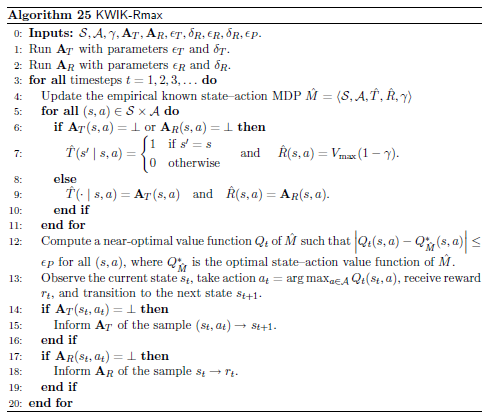
\includegraphics[width=0.6\textwidth]{kwik-rmax.png}
			\caption{kwik-rmax}
		\end{figure}

\paragraph{}En el algoritmo, es la l�nea 12 donde se decide la pr�xima acci�n. En la l�nea 13 obtenemos el reward y el estado siguiente, valores que se usan a continuaci�n para la fase de aprendizaje. \textbf{$A_T$} y \textbf{$A_R$} son los algoritmos que, dado un par estado-acci�n, determinan, respectivamente, el valor emp�rico de la probabilidad de moverse al estado deseado y el valor emp�rico del reward esperado, o, si no tienen suficientes datos, dicen que dicho par estado-acci�n es desconocido. Con una cota suficientemente grande, se garantiza que dicho algoritmo sea PAC dados $\epsilon$ y $\delta$. En la secci�n 7.2.1, p�gina 148, Li da un valor para esta cota (donde $n$ es la cantidad de estados y $m$ la cantidad de acciones):

\[
	O(\frac{n^2m}{\epsilon^2}ln(\frac{nm}{\delta}))
\]

\paragraph{}Sin embargo, en nuestro caso, tenemos el problema de la gran cantidad de estados posibles: En el tablero de 5 x 5 (el tablero utilizado para todas las pruebas) tenemos: 21 casilleros posibles para el agente, 21 casilleros posibles para la bomba, $2^5$ estados de paredes explotadas. Lo que da un total de 21 x 21 x 32 = 14112 estados. Entonces, asumiendo $\epsilon = 1$ y $\gamma = 1$, la cuenta de la cota igualmente es la siguiente (recordar que tenemos 6 acciones posibles):
\[
	14000^2\cdot6\cdot ln(14000\cdot6) =
\]

\subsubsection{RMax Factorizado}


	\subsubsection{Dyna-Q}
		
		
\paragraph{}Asumamos que tenemos un modelo del ambiente, esto es, que podemos predecir el siguiente estado y la recompensa dado un estado y una acci�n. La predicci�n puede ser un conjunto de posibles estados con su probabilidad asociada o puede ser un estado que es muestreado de acuerdo a la distribuci�n de probabilidad de los estados resultantes. Dado un modelo, es posible hacer planificaci�n. Lo interesante es que podemos utilizar los estados y acciones utilizados en la planificaci�n tambi�n para aprender. De hecho al sistema de aprendizaje no le importa si los pares estado-acci�n son dados de experiencias reales o simuladas. Dado un modelo del ambiente, uno podr�a seleccionar aleatoriamente un par (estado,acci�n), usar el modelo para predecir el siguiente estado, obtener una recompensa y actualizar valores Q. Esto se puede repetir indefinidamente hasta converger a Q\*.

\paragraph{}El algoritmo Dyna-Q combina experiencias con planificaci�n para aprender m�s r�pidamente una pol�tica �ptima.
La idea es aprender de experiencia, pero tambi�n usar un modelo para simular experiencia adicional y as� aprender m�s r�pidamente 

\paragraph{}El algoritmo de Dyna-Q selecciona pares estado-acci�n aleatoriamente de pares anteriores. Sin embargo, la planificaci�n se puede usar mucho mejor si se enfoca a pares estado-acci�n espec�ficos. Por ejemplo, enfocarnos en las metas e irnos hacia atr�s o m�s generalmente, irnos hacia atr�s de cualquier estado que cambie su valor.Los cambios en las estimaciones de valor V o Q pueden cambiar, cuando se est� aprendiendo o si el ambiente cambia y un valor estimado deja de ser cierto.

\paragraph{}Veamos el pseudoc�digo:
		
		\begin{figure}[h!]
			\centering
			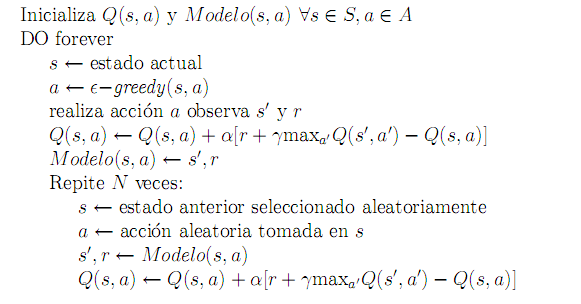
\includegraphics[width=0.6\textwidth]{Dyna.png}
			\caption{Algoritmo Dyna-Q}
		\end{figure}

\paragraph{}En nuestro casos los valores utilizados fueron:

\begin{itemize}
	
	\item N = 50 
	\item LEARNING\_RATE $= \alpha = 0.8 $
	\item DISCOUNT\_FACTOR $= \delta = 0.95 $
\end{itemize}	
	